\chapter{Υλοποίηση Του Αλγορίθμου}
\begin{sloppypar}
Ο αλγόριθμος αποτελείται από την κλάση \lstinline!HeuristicPlayer! στην οποία υλοποιούνται οι
συναρτήσεις  \lstinline!getNextMove()!,
\lstinline!getEvaluation()! (οι οποίες ζητούνται από την εκφώνηση) και η
\lstinline!calculateRisk()! (μία δίκη μας συνάρτηση, βοηθητική στην \lstinline!getEvaluation()!).
Με τις συναρτήσεις αυτές, αρχικά, αξιολογούμε την θέση.
Αυτό γίνεται με την \lstinline!calculateRisk()! και την
\lstinline!getEvaluation()!.
Αντλώντας πληροφορίες για τους γείτονες, τις διαθέσιμες τιμές που είναι
πιθανό να έρθουν για την επόμενη κίνηση  για τον αντίπαλο (και για εμάς) και τον αριθμό
των γειτονικών tiles των γειτόνων μας,
βρίσκουμε έναν αριθμό που αξιολογεί κάθε κενή θέση στο ταμπλό
(δηλαδή κάθε πιθανή επόμενη θέση μας).
Όσο μεγαλύτερος ο αριθμός, τόσο ευνοϊκότερη η θέση.
Στη συνέχεια με την συνάρτηση \lstinline!getNetMove()! βρίσκουμε τη
θέση με το μεγαλύτερο αριθμό αξιολόγησης και έπειτα τοποθετούμε το στρατό μας σε αυτή.
Επίσης,στην κλάση υπάρχουν, ήδη, υλοποιημένοι οι constructors.
Τέλος, να σημειωθεί ότι δημιουργήσαμε, μία ακόμη επιπλέον, συνάρτηση την \lstinline!updateOpponentsPool()! για να
παρακολουθούμε τις διαθέσιμες κινήσεις του αντιπάλου.
\end{sloppypar}

\section{Συνάρτηση \texttt{calculateRisk()}} \label{sec:calculateRisk}
\begin{lstlisting}[numbers=none, breaklines=true, title={Declaration της συνάρτησης}]
private double calculateRisk(final Tile tile, final Board board, final int nextTileScore)
\end{lstlisting}
Η συνάρτηση αυτή δέχεται ως ορίσματα ένα αντικείμενο τύπου \lstinline!Tile!,
ένα αντικείμενο τύπου \lstinline!Board! και
την μεταβλητή \lstinline!nextTileScore! που είναι το score του πλακιδίου που πρέπει να παίξουμε.
Επιστρέφει έναν \lstinline!double! με το κομμάτι του evaluation που αντιστοιχεί στην "ασφάλεια" της κίνησης.
Αυτό εξαρτάται από τους εξής παράγοντες:
\begin{enumerate}
\item Κατά πόσο το πλακίδιο που τοποθετούμε καλύπτεται από άλλα πλακίδια.
Αν έχει λίγους γείτονες μπορεί να κλαπεί πιο εύκολα από τον αντίπαλο.
\item Κατά πόσο βελτιώνεται ο βαθμός κάλυψης των γειτονικών φιλικών πλακιδίων.
Πχ αν πρέπει να παίξουμε ένα πλακίδιο με score $1$ μπορούμε να το τοποθετήσουμε σε τέτοια θέση που "κλείνει" ένα γειτονικό, φιλικό πλακίδιο με score $10$.
\item Κατά πόσο βελτιώνεται ο βαθμός κάλυψης των γειτονικών εχθρικών πλακιδίων.
Αν τοποθετήσουμε το πλακίδιο μας δίπλα σε ένα εχθρικό το οποίο δεν μπορούμε να το κλέψουμε τώρα, γίνεται πιο δύσκολο να το κλέψουμε αργότερα.
\end{enumerate}

Η δομή της συνάρτησης είναι η εξής:
\begin{itemize}
\item Το όρισμα \lstinline!tile! είναι το πλακίδιο για το οποίο πρέπει να υπολογίσουμε την ασφάλεια της τρέχουσας κίνησης.
\begin{enumerate}
\item \label{tile:isEnemyBigger}
Αν το \lstinline!tile! είναι του αντιπάλου και δεν είναι μικρότερο από το δικό μας, ο υπολογισμός γίνεται σύμφωνα με τα εναπομείναντα πλακίδια μας (\lstinline!myPool!).

\item \label{tile:tileIdMy}
Αν το \lstinline!tile! είναι δικό μας ή θα γίνει δικό μας,
ο υπολογισμός γίνεται σύμφωνα με τα εναπομείναντα πλακίδια του αντιπάλου (\lstinline!opponentsPool!).

\item \label{tile:tileId0}
Αν το \lstinline!tile! είναι άδειο, υπολογίζουμε την ασφάλεια για την τοποθέτηση πλακιδίου με score
\lstinline!nextTileScore! σε αυτή τη θέση πάλι σύμφωνα με τα εναπομείναντα πλακίδια του αντιπάλου (\lstinline!opponentsPool!).

\end{enumerate}
\begin{lstlisting}[numbers=none, aboveskip=\smallskipamount, belowskip=\smallskipamount, captionpos=none]
HashMap<Integer, Integer> map;
final int tileId = tile.getPlayerId();
final boolean isEmpty = (tileId == 0);
final double scoreTile = isEmpty ? nextTileScore : tile.getScore();
final boolean isEnemyBigger = (tileId == opponentId && nextTileScore <= scoreTile);
if (isEnemyBigger) {
    map = myPool;
} else {
    map = opponentsPool;
}
\end{lstlisting}

\item Βρίσκουμε τον αριθμό των κενών γειτόνων γύρω από το \lstinline!tile!.
Το άθροισμα στην
\hyperref[tile:tileId0]{περίπτωση}
που το \lstinline!tile! είναι άδειο αρχίζει από το \lstinline!1!.
\begin{lstlisting}[numbers=none, aboveskip=\smallskipamount, belowskip=\smallskipamount, captionpos=none]
final Tile[] neighbors = ProximityUtilities.getNeighbors(tile.getX(), tile.getY(), board);
double emptyNeighbors = isEmpty ? 1 : 0;
for (final Tile neighbor : neighbors) {
    if (neighbor != null && neighbor.getPlayerId() == 0) {
        emptyNeighbors++;
    }
}
\end{lstlisting}

\item Υπολογίζουμε από το \lstinline!map! τον αριθμό των πλακιδίων με μεγαλύτερο score από το \lstinline!tile! μας και τον συνολικό αριθμό των πλακιδίων.
\begin{lstlisting}[numbers=none, aboveskip=\smallskipamount, belowskip=\smallskipamount, captionpos=none]
double totalValuesCount = 0;
double biggerValuesCount = 0;
for (final Map.Entry<Integer, Integer> entry : map.entrySet()) {
    final Integer tileValue = entry.getKey();
    final Integer tileCount = entry.getValue();
    totalValuesCount += tileCount;
    if (tileValue > scoreTile) {
        biggerValuesCount += tileCount;
    }
}
if (totalValuesCount == 0) {
    return 0;
}
\end{lstlisting}

\item Υπολογίζουμε την "ασφάλεια" (\lstinline!risk!) του πλακιδίου σύμφωνα με τον τύπο μας.
\begin{lstlisting}[numbers=none, aboveskip=\smallskipamount, belowskip=\smallskipamount, captionpos=none]
final double percentLarger = biggerValuesCount / totalValuesCount;
final double risk = 2 * percentLarger * (scoreTile) / (emptyNeighbors * emptyNeighbors);
\end{lstlisting}
Κατασκευάσαμε δύο πιθανούς τύπους για τον υπολογισμό του \lstinline!risk!:
% Dunno if lstinline inside equation enviroment is a good idea.
% The log doesn't show anything concerning though.
\begin{equation}\label{eq:11}
\lstinline[basicstyle=\ttfamily]!risk! =
\frac{
    \frac{
        \lstinline[basicstyle=\ttfamily]!biggerValuesCount!
    }
    {
        \lstinline[basicstyle=\ttfamily]!totalValuesCount!
    } \cdot \lstinline[basicstyle=\ttfamily]!scoreTile!
}{
    \lstinline[basicstyle=\ttfamily]!emptyNeighbors!
}
\end{equation}
ή
\begin{equation}\label{eq:22}
\lstinline[basicstyle=\ttfamily]!risk! =
2 \cdot
\frac{
    \frac{
        \lstinline[basicstyle=\ttfamily]!biggerValuesCount!
    }
    {
        \lstinline[basicstyle=\ttfamily]!totalValuesCount!
    } \cdot \lstinline[basicstyle=\ttfamily]!scoreTile!
}{
    \lstinline[basicstyle=\ttfamily]!emptyNeighbors!^2
}
\end{equation}

Η λογική και των δύο είναι παρόμοια. Ο λόγος: \[
P = \frac{
    \lstinline[basicstyle=\ttfamily]!biggerValuesCount!
}
{
    \lstinline[basicstyle=\ttfamily]!totalValuesCount!
}
\] δηλώνει την πιθανότητα να κληρωθεί στον αντίπαλο πλακίδιο με μεγαλύτερο score από το \lstinline!tile!.
Το γινόμενό του με το \lstinline!scoreTile!: \[
P \cdot \lstinline[basicstyle=\ttfamily]!scoreTile!
\] αντιπροσωπεύει το προσδόκιμο αριθμό πόντων που μπορεί να κλέψει ένας παίκτης αν επιλέξει να παίξει σε ένα από τα γειτονικά πλακίδια του \lstinline!tile!.
Έπειτα, προσπαθούμε να περιορίσουμε αυτόν τον αριθμό σύμφωνα με τον αριθμό των κενών γειτόνων.
Όσο πιο πολλούς κενούς γείτονες έχει το \lstinline!tile! τόσο λιγότερο νόημα έχει να προσπαθήσουμε να το καλύψουμε.
Σε αυτό το σημείο βρίσκεται η διαφορά των δύο τύπων:
\begin{itemize}
\item Στον \hyperref[eq:11]{\ref{eq:11}}
διαιρούμε απλώς με το \lstinline!emptyNeighbors!.

\item Στον \hyperref[eq:22]{\ref{eq:22}}
διαιρούμε με το τετράγωνο του \lstinline!emptyNeighbors! και πολλαπλασιάζουμε το τελικό αποτέλεσμα με το $2$.
Αυτό έχει ως σκοπό την μεγαλύτερη μείωση του \lstinline!risk! σε πλακίδια με πολλούς γείτονες.
Ο πολλαπλασιασμός με το $2$ αποσκοπεί στην αύξηση του συντελεστή ώστε να μην γίνει πολύ μικρός.
Ο συντελεστής αυτός βρέθηκε πειραματικά μετά από αρκετές δοκιμές.
\end{itemize}

Μετά από αρκετά πειράματα αποφασίσαμε ότι ο τύπος \hyperref[eq:22]{\ref{eq:22}} είναι καλύτερος και για αυτό χρησιμοποιούμε αυτόν στην τελική έκδοση.
\noindent\begin{center}
    \selectlanguage{greek}
    \centering
    \noindent\begin{minipage}{\textwidth}
        \centering
        \captionsetup{type={figure}}
        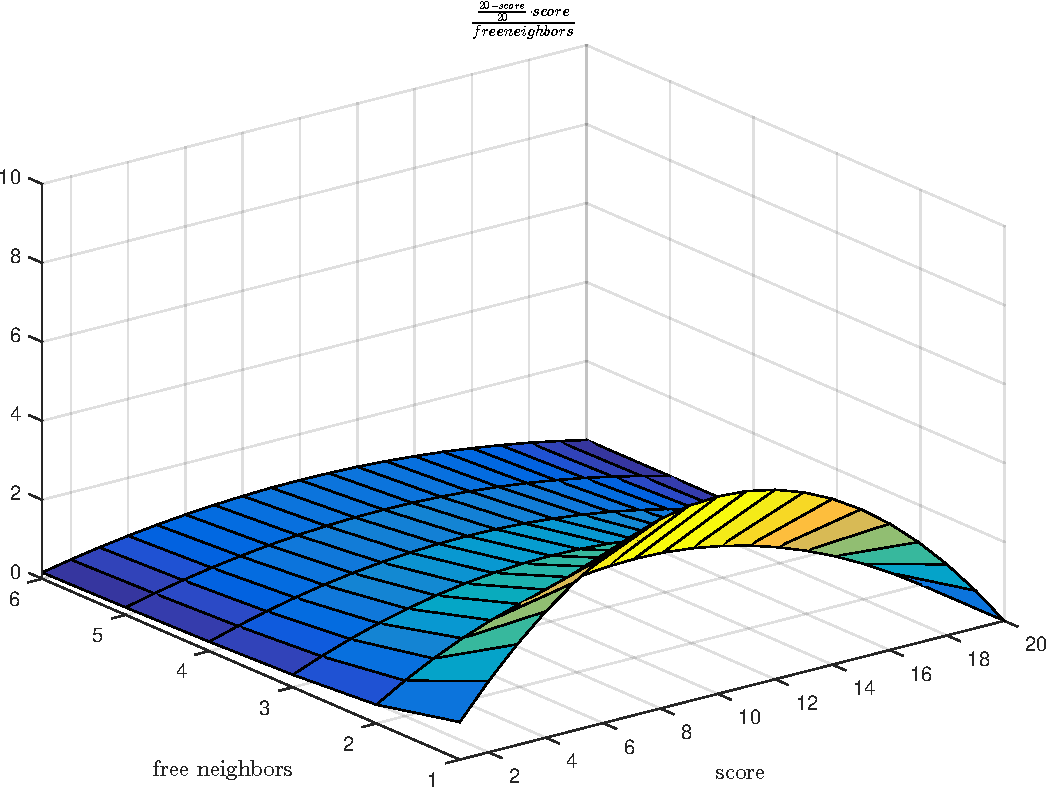
\includegraphics[height=0.45\textheight]{img/11.pdf}
        \captionof{figure}{Γράφημα του \ref{eq:11} στην αρχή του παιχνιδιού}
    \end{minipage} %
    \vfill
    \noindent\begin{minipage}{\textwidth}
        \centering
        \captionsetup{type={figure}}
        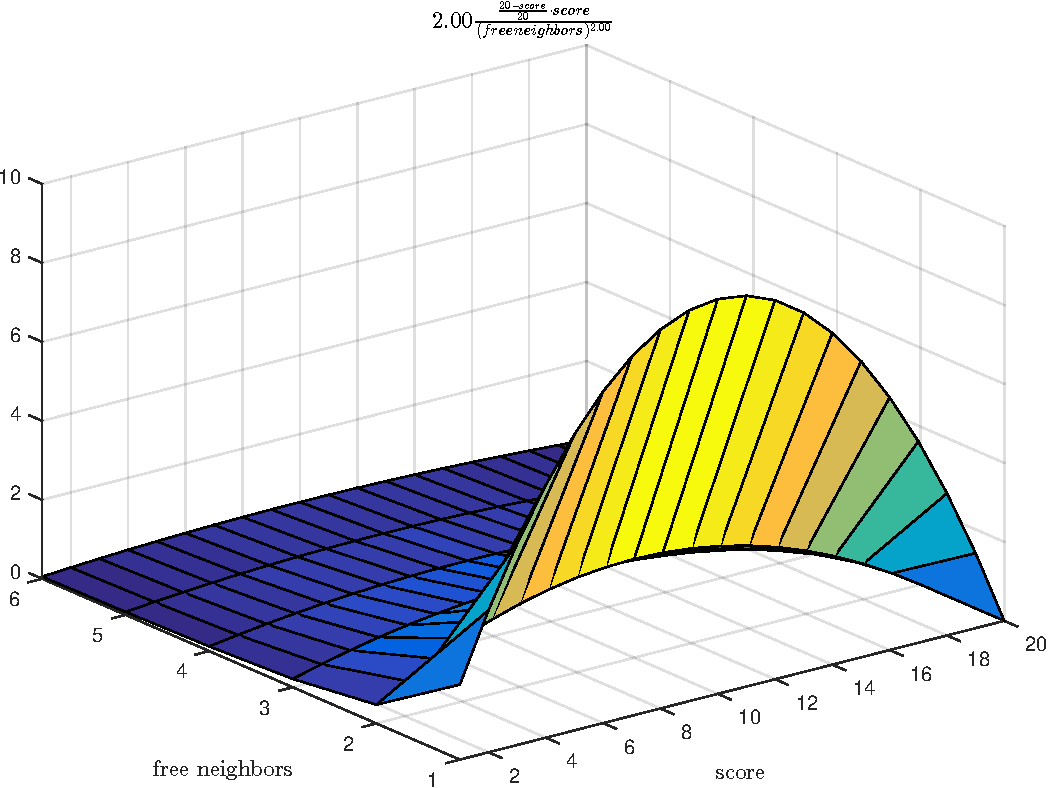
\includegraphics[height=0.45\textheight]{img/22.pdf}
        \captionof{figure}{Γράφημα του \ref{eq:22} στην αρχή του παιχνιδιού}
    \end{minipage} %
\end{center}

\item Επιστρέφουμε \lstinline!-risk! αν το \lstinline!tile! είναι του αντιπάλου και μεγαλύτερο από το
\lstinline!nextTileScore! (καθώς βελτιώνουμε την θέση του).
Αλλιώς, επιστρέφουμε \lstinline!risk!.
\begin{lstlisting}[numbers=none, aboveskip=\smallskipamount, belowskip=\smallskipamount, captionpos=none]
if (isEnemyBigger) {
    return -risk;
} else {
    return risk;
}
\end{lstlisting}
\end{itemize}

\section{Συνάρτηση \texttt{getEvaluation()}}
\begin{lstlisting}[numbers=none, title={Declaration της συνάρτησης}]
public double getEvaluation(final Board board, final int randomNumber, final Tile tile)
\end{lstlisting}
Η συνάρτηση αυτή δέχεται ως ορίσματα ένα αντικείμενο τύπου \lstinline!Board!, την μεταβλητή
\lstinline!randomNumber! και ένα αντικείμενο τύπου \lstinline!Tile! και επιστρέφει
μία μεταβλητή τύπου \lstinline!double!.

Η δομή της συνάρτησης είναι η εξής:\begin{itemize}
\item Καλούμε τη συνάρτηση \lstinline!getNeigbhors()! για τις συντεταγμένες του \lstinline!tile! και αποθηκεύουμε σε έναν πίνακα \lstinline!Tile[] neighbors!,
τον επιστρεφόμενο πίνακα της συνάρτησης \lstinline!ProximityUtilities.getNeigbhors()! που περιέχει τους γείτονες του πλακιδίου \lstinline!tile!.
\begin{lstlisting}[numbers=none, aboveskip=\smallskipamount, belowskip=\smallskipamount, captionpos=none]
final Tile[] neighbors = ProximityUtilities.getNeighbors(tile.getX(), tile.getY(), board);
\end{lstlisting}

\item Καλούμε τη συνάρτηση \lstinline!calculateRisk()! η οποία αναλύεται στο
\hyperref[sec:calculateRisk]{\ref{sec:calculateRisk}}
και η οποία επιστρέφει μία την τιμή "ασφάλειας" για την τοποθέτηση του \lstinline!randomNumber!
στο \lstinline!tile!.

\item Αρχή μιας \lstinline!for! η οποία παίρνει ένα-ένα τους γείτονες του \lstinline!tile!.
\begin{lstlisting}[numbers=none, aboveskip=\smallskipamount, belowskip=\smallskipamount, captionpos=none]
for (final Tile neighbor : neighbors) {
\end{lstlisting}

\item Αν ένας γείτονας είναι κενός ή \lstinline!null! τότε πηγαίνουμε στον επόμενο γείτονα.
\begin{lstlisting}[numbers=none, aboveskip=\smallskipamount, belowskip=\smallskipamount, captionpos=none]
if (neighbor == null || neighbor.getPlayerId() == 0) {
    continue;
}
\end{lstlisting}

\item Αποθηκεύουμε σε μία μεταβλητή το id του γείτονα και σε μία δεύτερη μεταβλητή το score του.
\begin{lstlisting}[numbers=none, aboveskip=\smallskipamount, belowskip=\smallskipamount, captionpos=none]
final int neighborPlayerId = neighbor.getPlayerId();
final int neighborScore = neighbor.getScore();
\end{lstlisting}

\item \begin{sloppypar}Αν το πλακίδιο ανήκει σε αντίπαλο και ο \lstinline!randomNumber! είναι μεγαλύτερος από το score του πλακιδίου του γείτονα τότε προσθέτουμε στη μεταβλητή \lstinline!scoreFromEnemies!
(μεταβλητή που αρχικοποιημένη στη τιμή \lstinline!0!) το σκορ του αντιπάλου.\end{sloppypar}
\begin{lstlisting}[numbers=none, aboveskip=\smallskipamount, belowskip=\smallskipamount, captionpos=none]
if (neighborPlayerId == opponentId && randomNumber > neighborScore) {
    scoreFromEnemies += neighborScore;
}
\end{lstlisting}

\item Αλλιώς, αν το πλακίδιο είναι δικό μας και το σκορ του γειτονικού πλακιδίου
δεν είναι \lstinline!20! τότε αυξάνουμε έναν μετρητή
(αρχικοποιημένο στο \lstinline!0!) κατά \lstinline!1!.
\begin{lstlisting}[numbers=none, aboveskip=\smallskipamount, belowskip=\smallskipamount, captionpos=none]
else if (neighborPlayerId == id && neighborScore != 20) {
    scoreFromAlies++;
}
\end{lstlisting}

\item Προσθέτουμε στο \lstinline!scoreFromRisk! την επιστρεφόμενη τιμή της \lstinline!calculateRisk()!
\begin{lstlisting}[numbers=none, aboveskip=\smallskipamount, belowskip=\smallskipamount, captionpos=none]
scoreFromRisk += calculateRisk(neighbor, board, randomNumber);
\end{lstlisting}

\item Η επιστρεφόμενη τιμή της συνάρτησης είναι το άθροισμα
\lstinline!scoreFromAlies + scoreFromEnemies + scoreFromRisk!.
Ουσιαστικά, με τη λούπα βρίσκουμε για κάθε πιθανή θέση, πόσο σκορ θα κερδίζαμε αν τοποθετούσαμε το πλακίδιο μας εκεί.
Ωστόσο, πέρα από το συνολικό σκορ που κερδίζουμε σε κάθε θέση υπάρχουν και άλλοι
παράγοντες που επηρεάζουν την τελική επίδοση μας (πχ πόσο προστατευμένοι είμαστε, πόσο εύκολα μπορεί να μας πάρει το στρατό ο αντίπαλος κτλ) και για αυτό χρησιμοποιεί η \lstinline!calculateRisk()!
\end{itemize}

\section{Συνάρτηση \texttt{getNextMove()}}
\begin{lstlisting}[numbers=none, title={Declaration της συνάρτησης}]
public int[] getNextMove(final Board board, final int randomNumber)
\end{lstlisting}
Η συνάρτηση αυτή δέχεται ως ορίσματα ένα αντικείμενο τύπου \lstinline!Board! και
την μεταβλητή \lstinline!randomNumber! και επιστρέφει έναν
μονοδιάστατο πίνακα(\lstinline!result[3]!) με τις συντεταγμένες \lstinline!x,y!
που αντιστοιχούν στην θέση με την καλύτερη αξιολόγηση καθώς και τον
\lstinline!randomNumber!.

Η δομή της συνάρτησης είναι η εξής:\begin{itemize}
\item Καλούμε τη συνάρτηση\lstinline!updateOpponentPool()! την
οποία αναλύουμε στο \hyperref[sec:updateOpponentsPool]{\ref{sec:updateOpponentsPool}}

\item Καλούμε τη συνάρτηση \lstinline!getMyPool()! η οποία επιστρέφει ένα αντικείμενο τύπου \lstinline!HashMap! που αναπαριστά το σύνολο των διαθέσιμων τιμών που είναι πιθανό να έρθουν για την επόμενη κίνηση
\begin{lstlisting}[numbers=none, aboveskip=\smallskipamount, belowskip=\smallskipamount, captionpos=none]
myPool = board.getMyPool();
\end{lstlisting}

\item Αρχή μιας λούπας που προσπελάζει κάθε διαφορετικό πλακίδιο στο ταμπλό
\begin{lstlisting}[numbers=none, aboveskip=\smallskipamount, belowskip=\smallskipamount, captionpos=none]
for (int i = 0; i < ProximityUtilities.NUMBER_OF_ROWS; i++) {
    for (int j = 0; j < ProximityUtilities.NUMBER_OF_COLUMNS; j++) {
\end{lstlisting}

\item Σε κάθε επανάληψη της καλούμε την συνάρτηση \lstinline!board.getTile()! που επιστρέφει ένα αντικείμενο τύπου \lstinline!Tile!. Αυτό είναι το πλακίδιο στη θέση \lstinline!j,i!.
\begin{lstlisting}[numbers=none, aboveskip=\smallskipamount, belowskip=\smallskipamount, captionpos=none]
final Tile tile = board.getTile(j, i);
\end{lstlisting}

\item Αν η θέση είναι κενή (άρα μπορούμε να τοποθετήσουμε το νέο μας πλακίδιο εκεί),
τότε καλούμε την \lstinline!getEvaluation()! και αποθηκεύουμε την επιστρεφόμενη τιμή
στην μεταβλητή \lstinline!evaluation!.
\begin{lstlisting}[breaklines=true, numbers=none, aboveskip=\smallskipamount, belowskip=\smallskipamount, captionpos=none]
if (tile.getPlayerId() == 0) {
    final double evaluation = getEvaluation(board, randomNumber, tile);
\end{lstlisting}

\item Αν η \lstinline!evaluation! είναι μεγαλύτερη της
\lstinline!max! (μία μεταβλητή την οποία έχουμε αρχικοποιήσει αρχικά στη τιμή \lstinline!Double.NEGATIVE_INFINITY!) αποθηκεύουμε
τις συντεταγμένες του πλακιδίου στον πίνακα \lstinline!result!.
\begin{lstlisting}[breaklines=true, numbers=none, aboveskip=\smallskipamount, belowskip=\smallskipamount, captionpos=none]
if (evaluation >= max) {
    max = evaluation;
    result[0] = tile.getX();
    result[1] = tile.getY();
}
\end{lstlisting}

\item \begin{sloppypar}Όταν τελειώσει η \lstinline!for! θα έχουμε αποθηκευμένο στη \lstinline!max! το μεγαλύτερο \lstinline!evaluation! και στον πίνακα \lstinline!result! τις
αντίστοιχες συντεταγμένες του πλακιδίου με το μεγαλύτερο \lstinline!evaluation!.\end{sloppypar}

\item Τοποθετούμε στη τρίτη θέση του πίνακα result το \lstinline!randomNumber!.
\begin{lstlisting}[breaklines=true, numbers=none, aboveskip=\smallskipamount, belowskip=\smallskipamount, captionpos=none]
result[2] = randomNumber;
\end{lstlisting}

\item Επιστρέφουμε τον πίνακα \lstinline!result!.
\end{itemize}

\section{Συνάρτηση \texttt{updateOpponentsPool()}} \label{sec:updateOpponentsPool}
\begin{lstlisting}[numbers=none, title={Declaration της συνάρτησης}]
private void updateOpponentsPool(final Board board)
\end{lstlisting}
Η συνάρτηση αυτή δέχεται ως όρισμα ένα αντικείμενο τύπου \lstinline!Board!,
δεν επιστρέφει τίποτα και
ενημερώνει την \lstinline!self.opponentsPool! με τις εναπομείναντες κινήσεις του αντίπαλου παίκτη.
\begin{lstlisting}[numbers=none, breaklines=true, title={Declaration της \lstinline!opponentsPool!}]
private final HashMap<Integer, Integer> opponentsPool = new HashMap<Integer, Integer>();
\end{lstlisting}

Η δομή της συνάρτησης είναι η εξής:
\begin{itemize}
\item Παίρνουμε την τελευταία κίνηση του αντιπάλου.
\begin{lstlisting}[breaklines=true, numbers=none, aboveskip=\smallskipamount, belowskip=\smallskipamount, captionpos=none]
final int[] lastMove = board.getOpponentsLastMove();
\end{lstlisting}

\item Αν το αποτέλεσμα περιέχει \lstinline!-1! τότε σημαίνει ότι ο αντίπαλος δεν έχει παίξει ακόμα οπότε η συνάρτηση επιστρέφει

\item Παίρνουμε το \lstinline!Tile! που αντιστοιχεί στην τελευταία κίνηση.
\begin{lstlisting}[breaklines=true, numbers=none, aboveskip=\smallskipamount, belowskip=\smallskipamount, captionpos=none]
final Tile lastMoveTile = board.getTile(lastMove[0], lastMove[1]);
\end{lstlisting}

\item Χρησιμοποιούμε ως \lstinline!key! στο \lstinline!HashMap! μας το score του αντίπαλου πλακιδίου.
Θεωρούμε ότι, σύμφωνα με τους κανόνες, το \lstinline!Tile! στην θέση που έπαιξε τον προηγούμενο γύρο ο αντίπαλος έχει το ίδιο score με το πλακίδιο που του κληρώθηκε στην προηγούμενη κίνηση.
Έτσι, αφαιρούμε τα εναπομείναντα πλακίδια αυτού του score κατά \lstinline!1!
\begin{lstlisting}[breaklines=true, numbers=none, aboveskip=\smallskipamount, belowskip=\smallskipamount, captionpos=none]
final Integer key = lastMoveTile.getScore();
// decrease by 1.
final Integer value = opponentsPool.get(key) - 1;
opponentsPool.put(key, value);
\end{lstlisting}

\item Ανανεώνουμε το \lstinline!opponentsPool! και η συνάρτηση επιστρέφει.
\begin{lstlisting}[breaklines=true, numbers=none, aboveskip=\smallskipamount, belowskip=\smallskipamount, captionpos=none]
opponentsPool.put(key, value);
\end{lstlisting}
\end{itemize}

Σημειώνεται ότι το \lstinline!opponentsPool! αρχικοποιείται με \lstinline!3! κινήσεις για κάθε score πλακιδίου στον constructor.
\begin{lstlisting}[breaklines=true, numbers=none, aboveskip=\smallskipamount, belowskip=\smallskipamount, captionpos=none]
for (Integer key = 1; key <= 20; key++) {
    opponentsPool.put(key, 3);
}
\end{lstlisting}
